\documentclass[a4paper,12pt,reqno]{amsart}
\usepackage{M67tds}

% pour voir les solutions il faut enlever le commentaire de la ligne suivante
% \solutionstrue

\newlist{axioms}{description}{1}
\newcommand\axiomlabel[1]{\hfill\textbf{(#1)}}
\setlist[axioms]{style=nextline,before={\let\makelabel\axiomlabel}}
\newcommand*{\ensemble}[3][]{#1\{ #2 \;#1|\; #3 #1\}} % par exemple \ensemble[\big]{x^2}{x \in \R}
\newcommand*{\abs}[1]{\left\lvert{\ifx\hfuzz#1\hfuzz \,\cdot\,\else#1\fi}\right\rvert} % la valeur absolue
\newcommand*{\axiom}[1]{\textbf{(#1)}}
\newcommand*{\overeq}[1]{\overset{\tiny{#1}}{=}}

% raccourcis
\DeclareMathOperator{\A}{aire}

% Les notes de bas de page dans les minipages (sidebyside)
\renewcommand{\thempfootnote}{\fnsymbol{mpfootnote}}

% pour surligner
\sisolutions{
  \usepackage{soul}
  \colorlet{hl}{yellow!35!white}
  \sethlcolor{hl}
}

\begin{document}

% ==================================
\hautdepage{

\ifsolutions{Solutions du rattrapage}\else{Rattrapage}\fi\par\normalfont\normalsize
21 juin 2019\\{[ durée: 3 heures ]}\par
}
% ==================================
\sisujet{
  % {\fontencoding{U}\fontfamily{futs}\selectfont\char 66\relax}
  \tikz[baseline=(e.base)]{\NoAutoSpacing\node(e){!};\draw[red,ultra thick,line join=round,yshift=-.15ex](90:1em)--(210:1em)--(330:1em)--cycle;}
  \textbf{Documents autorisés :}\textit{Une feuille A4 recto-verso écrite à la main.}

  \vspace{17mm}
  \tsvp
}




%-----------------------------------
\begin{exo} (Construction à la règle et compas)

  \sidebyside{.7}{
    \begin{enumerate}
      \item Soient $A_{1}$ et $A_{2}$ deux points distincts du plan. Construire à la règle et au compas (en rédigeant le programme de construction choisi) les sommets $A_1, A_2, \ldots, A_8$ d'un octogone régulier\footnotemark{} ayant $A_{1}A_{2}$ pour côté.
      \item Déterminer l'aire de cet octogone régulier en fonction de la longueur $a=A_{1}A_{2}$.
    \end{enumerate}
  }{
    \raisebox{-35mm}[0pt][0pt]{\includegraphics[width=4cm]{M67_2018-19_Rattrapage_img_octogone}}
  }
  \footnotetext{Octogone convexe dont les côtés ont tous la même longueur.}
\end{exo}

\begin{solution}\def\C{\mathcal{C}}
  \begin{enumerate}
    \item
    On va donner la construction à la règle et au compas du point $A_{i+1}$ à partir des points $A_{i-1}$ et $A_{i}$. Ce point est tel que $\widehat{A_{i+1} A_i A_{i-1}} = 135°$ et $A_{i+1} A_i = A_{i-1} A_{i}$. Pour cela on va d'abord construire un point $S$ qui est tel que $SA_{i-1}A_{i}$ soit un triangle rectangle isocèle.

    \sidebyside{.7}{
      \begin{convention}
        On note $\C(X,Y)$ le cercle de centre $X$ passant par $Y$, et $\C^{*}(X,Y) = \C(X,Y)\setminus\{Y\}$.
      \end{convention}
      \begin{enumerate}[1.]
        \item $P=\C^*(A_{i-1},A_i) \cap (A_iA_{i-1})$;
        \item $\{Q,R\}=\C(A_i,P) \cap \C(P,A_i)$;
        \item $\{S,T\}=\C(A_{i-1},A_i) \cap (QR)$;
        \item $A_{i+1}=\C(A_{i},A_{i-1}) \cap (SA_i)$.
      \end{enumerate}
      Ainsi successivement on construit $A_{3}$ à partir de $A_{1}$ et $A_{2}$, puis $A_{4}$ à partir de $A_{2}$ et $A_{3}$ et ainsi de suite jusqu'à $A_{8}$.
    }{
      \raisebox{-53mm}[0pt][0mm]{\includegraphics[width=5cm]{M67_2018-19_Rattrapage_img_construction_octogone}}
    }
    \item
    \sidebyside{.7}{
      L'aire d'un octogone de côté $a$ est obtenue à partir de l'aire d'un carré de côté $(1+\sqrt{2})a$ auquel on retranche quatre demi-carrés de côté $\frac{a}{\sqrt{2}}$ (voir la figure ci-contre). Ainsi on trouve que l'aire recherchée est $(1+\sqrt{2})^2a^{2} - 2 \left(\frac{a}{\sqrt{2}} \right)^2 = 2(1+\sqrt{2})a^{2}$.
    }{
      \raisebox{-21mm}[0pt][0pt]{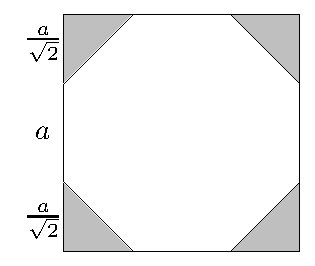
\includegraphics[width=3cm]{M67_2018-19_DS2_img_aire_octogone}}

    }
  \end{enumerate}
\end{solution}

\sisujet{\bigskip}
%-----------------------------------
\begin{exo} (Quadrilatère inscriptible et aire)

  \begin{enumerate}
    \item À quelle condition un parallélogramme $ABCD$ est-il inscrit dans un cercle\footnote{C.-à-d. a les quatre sommets sur un même cercle.}?
    \item Soit $\mathcal{C}$ un cercle de rayon $R$. Quelle est l'aire maximale d'un parallélogramme inscrit dans le cercle $\mathcal{C}$?
    \item Soit $\mathcal{C}$ un cercle de rayon $R$ et $ABCD$ un parallélogramme d'aire $S$ inscrit dans $\mathcal{C}$. Exprimer le périmètre $P$ de $ABCD$ en fonction du rayon $R$ et de l'aire $S$.
    \item Soit $\mathcal{C}$ un cercle de rayon $R$. Quel est le périmètre maximal d'un parallélogramme inscrit dans le cercle $\mathcal{C}$?
  \end{enumerate}
\end{exo}

\begin{solution}

  \begin{enumerate}
     \item Les angles opposés d'un parallélogramme sont égaux. D'autre part, les angles opposés d'un quadrilatère convexe inscrit dans un cercle sont supplémentaires. Un parallélogramme inscrit dans un cercle a donc ses angles droits, c'est un rectangle. Cette condition nécessaire est aussi suffisante car un rectangle est un parallélogramme inscrit dans un cercle.
     \item D'après la question précédente, un parallélogramme $ABCD$ inscrit dans un cercle est un rectangle. Ses diagonales $[AC]$ et $[BD]$ sont alors des diamètres du cercle. Si on note $\alpha \in [0,\pi/2] $ la mesure de l'angle (aigu) entre les diagonales, alors l'aire de $ABCD$ est $2R^{2}\sin(\alpha)$. Ainsi l'aire maximale de $ABCD$ est $2R^{2}$, et elle est atteinte quand $AC\perp BD$, autrement dit si et seulement si $ABCD$ est un carré.
     \item On note $a$ et $b$ les côtés du rectangle $ABCD$ ayant une diagonale de $2R$. D'après Pythagore $a^{2}+b^{2} = 4R^{2}$ et donc $P^{2} = 4(a+b)^{2} = 4(a^2+b^2) + 8ab = 16R^{2}+8S$. Et ainsi on trouve $P = \sqrt{16R^{2}+8S}$.
     \item D'après les deux questions précédentes on trouve que le périmètre est maximal quand l'aire est maximale, c.-à-d. quand $ABCD$ est un carré, et dans ce cas il vaut $P = 4\sqrt{2}R$.
  \end{enumerate}
\end{solution}

\newpage
%-----------------------------------
\begin{exo} (Triangles)

  \sidebyside{.77}{
    Soit $ABC$ un triangle. On considère le triangle $A'B'C'$ obtenu en prolongeant vers l'extérieur chaque côté de la moitié de sa longueur. Plus précisément, $A'$ est le point de $[CA)$ tel que $AA'=\frac{1}{2}CA$, $B'$ le point de $[AB)$ tel que $BB'=\frac{1}{2}AB$ et $C'$ le point de $[BC)$ tel que $CC'=\frac{1}{2}BC$.
  }{
    \raisebox{-28mm}[0pt][0pt]{\includegraphics[width=4cm]{M67_2018-19_Rattrapage_triangle}}
  }

  \begin{enumerate}
    \item Calculer l'aire de $A'B'C'$ en fonction de l'aire de $ABC$.
    \item Démontrer que la droite $(AC)$ coupe la droite $(B'C')$ en un point $M$ situé entre $B'$ et $C'$.
    \item Démontrer que $\displaystyle{\frac{C'M}{B'M}=\frac{1}{3}}$.
    \begin{indication}
      On peut utiliser le lemme dit « du chevron ».
    \end{indication}
    \item Expliquer comment retrouver le triangle d'origine $ABC$ à partir du triangle $A'B'C'$.
  \end{enumerate}
\end{exo}

\begin{solution}
  \begin{enumerate}
    \item Puisque $B$, $C$ et $C'$ sont alignés avec $CC'=\frac{1}{2} BC$, on a $\A(ACC')=\frac{1}{2}\A(ABC)$. Puisque $C$, $A$ et $A'$ sont alignés avec $CA'=\frac{3}{2}CA$, on a $\A(CC'A')=\frac{3}{2}\A(CC'A)=\frac{3}{4}\A(ABC)$.\\
    On montre de même que $\A(BCC')$ et $\A(AA'B')$ sont égales à $\frac{3}{4}\A(ABC)$.\\
    Finalement, $A'B'C'$ étant union presque disjointe des quatre triangles $ABC$, $BB'C'$, $CC'A'$ et $AA'B'$ on a $\A(A'B'C')=(1+3 \cdot \frac{3}{4})\A(ABC)=\frac{13}{4}\A(ABC)$.
    \item La droite $(AC)$ coupe la droite $(BC')$ en $C$ qui est entre $B$ et $C'$. Elle coupe la droite $(BB')$ en $A$ qui n'est pas entre $B$ et $B'$ (puisque c'est $B$ qui est entre $A$ et $B'$). D'après l'axiome de Pasch appliqué dans le triangle $BB'C'$, $(AC)$ coupe donc la droite $(B'C')$ entre $B'$ et $C'$, en un point noté $M$.
    \item D'après le lemme dit « du chevron », $\frac{C'M}{B'M}=\frac{\A(C'AA')}{\A(B'AA')}$. Or, d'après ce qui a été vu plus haut, $\A(C'AA')= \frac{1}{4}\A(ABC)$ et $\A(B'AA')=\frac{3}{4}\A(ABC)$. D'où le résultat.
    \item On a donc $\frac{C'M}{C'B'}=\frac{1}{4}$. On peut donc construire $M$ à partir de $B'$ et $C'$ en construisant d'abord le milieu de $[B'C']$ intersection de la droite $(B'C')$ et de la droite passant par les deux points d'intersection des cercles de centre $B'$ passant par $C'$ et de centre $C'$ passant par $B'$. On obtient ensuite  le milieu de $[C'I]$ comme intersection de $(B'C')$ et de la droite passant par les points d'intersection des deux cercles de rayon $[C'I]$. On construit de même le point $N$ de $(AC)$ tel que $A'N=\frac{1}{4} A'C'$, et le point $P$ de $(A'B')$ tel que $B'P=\frac{1}{4}B'A'$. On obtient finalement $A$ comme intersection de $(B'N)$ et $(A'M)$, $B$ de $(C'P)$ et $(B'N)$ et $C$ de $(A'M)$ et $(C'P)$.
  \end{enumerate}
\end{solution}

\sisujet{\bigskip}
%-----------------------------------
\begin{exo}[.7] (Kangourou 2005)

  \sidebyside{.7}{
    Dans le quadrilatère $JKLM$, la droite $(KM)$ est la bissectrice de $\widehat{JKL}$ et $JL=KL$. En sachant que $\widehat{KML}=80^{\circ}$ et $\widehat{JLK}=20^{\circ}$, que vaut l'angle $\widehat{KJM}$ ?
  }{
    \raisebox{-21mm}[0pt][0pt]{\includegraphics[width=5cm]{img_kangourou2005}}
  }
\end{exo}

\begin{solution}

  \sidebyside{.7}{
    Comme le triangle $\tri KLJ$ est isocèle, on trouve $\widehat{KJL} = \frac{1}{2}(180^{\circ}-20^{\circ}) = 80^{\circ}$. Donc les points $K,L,M,J$ sont cocycliques, car $\widehat{KJL} = \widehat{KML}$. Ainsi $\widehat{JLM} = \widehat{JKM} = \frac{1}{2}80^{\circ} = 40^{\circ}$. Et pour finir $\widehat{KJM} = 180^{\circ} - \widehat{KLM} = 180^{\circ} - 20^{\circ}-40^{\circ} = 120^{\circ}$.
  }{
    \raisebox{-28mm}[0pt][0pt]{\includegraphics[width=5cm]{img_kangourou2005s}}
  }
\end{solution}


\end{document}
